\documentclass{article}
\usepackage[margin = 0.15in,landscape]{geometry}
\usepackage{multicol}
\usepackage{array}
\usepackage{amsmath}
\usepackage{amssymb}
\usepackage{lmodern}
\usepackage{graphicx}
<<<<<<< HEAD
<<<<<<< HEAD
\usepackage{enumitem}
\setlength\parindent{0pt}
\renewcommand{\baselinestretch}{0.75}
=======

\setlength\parindent{0pt}
\renewcommand{\baselinestretch}{0.5}
>>>>>>> eefe2b0 (Begins Orbital Exam 1 crib sheet.)
=======
\usepackage{enumitem}
\setlength\parindent{0pt}
\renewcommand{\baselinestretch}{0.75}
>>>>>>> c99cbd9 (Finishes the different types of orbits and their properties.)


\begin{document}
\begin{multicols*}{3}
<<<<<<< HEAD
<<<<<<< HEAD
    Marissa Palamara\par 
    ASEN 3200\par 
    Fall 2020
    \vspace{-0.5cm}
    \setlist{nolistsep}
=======
>>>>>>> eefe2b0 (Begins Orbital Exam 1 crib sheet.)
=======
    \setlist{nolistsep}
>>>>>>> c99cbd9 (Finishes the different types of orbits and their properties.)
    \subsection*{Two-Body Problem}
    Newton's Law: $\Sigma \vec{F}=\frac{d(m\vec{v})}{dt}=m\vec{a}$ \par
    Universal Law of Gravitation: $\vec{F}_g=-\frac{Gm_1m_2}{r^2}\frac{\vec{r}}{|\vec{r}|}$\par 
    Apply Newton's Laws to a two-body problem with the assumptions:
    \begin{enumerate}
        \itemsep0em
        \item Only system force: Gravity $\rightarrow$ acts along the line joining the centers of the bodies.
        \item Mass of each body is constant.
        \item Treat each body as a spherically symmetrical point mass with uniform density.
    \end{enumerate}
<<<<<<< HEAD
<<<<<<< HEAD
    \subsection*{Orbits}
    \textbf{Elliptical Orbits}:\par
    \textbf{Orbital Properties:}
=======
    Orbital Properties:
>>>>>>> eefe2b0 (Begins Orbital Exam 1 crib sheet.)
=======
    \subsection*{Orbits}
    \textbf{Elliptical Orbits}:\par
    \textbf{Orbital Properties:}
>>>>>>> c99cbd9 (Finishes the different types of orbits and their properties.)
    \begin{itemize}
        \itemsep0em
        \item a = semimajor axis
        \item b = semiminor axis
        \item p = semiperimeter
        \item $r_a/r_p$ = radii of apoapsis/periapsis
        \item $\vec{e}$ = eccentricity
    \end{itemize}
    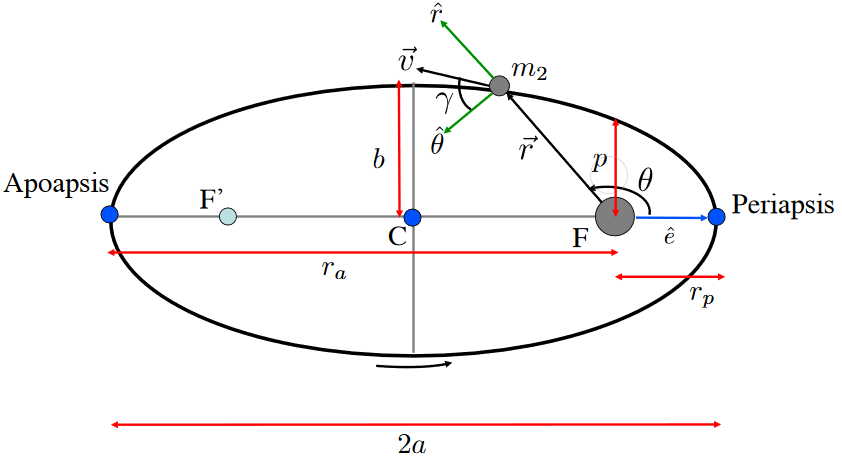
\includegraphics[width=\linewidth]{Figures/orbital_properties.png}
<<<<<<< HEAD
<<<<<<< HEAD

    \textbf{Useful Equations:}\par
=======
    Useful Equations:\par
>>>>>>> eefe2b0 (Begins Orbital Exam 1 crib sheet.)
=======

    \textbf{Useful Equations:}\par
>>>>>>> c99cbd9 (Finishes the different types of orbits and their properties.)
    $a = \frac{1}{2}(r_a+r_p)$\par 
    $p=\frac{b^2}{a}=a(1-e^2)=\frac{h^2}{\mu}$\par 
    $r_a = \frac{p}{1-e}=a(1+e)$\par 
    $r_p = \frac{p}{1+e}=a(1-e)$\par
    $e = \frac{r_a-r_p}{r_a+r_p}$ = $\frac{c}{a}$ = $\frac{\sqrt{a^2-b^2}}{a}$ = $\sqrt{1+\frac{2h^2\varepsilon}{\mu^2}}$\par 
    $b = a\sqrt{1-e^2}$ \par
    Angular Momentum: $\vec{h} = \vec{r} \times \vec{v}$ = $\sqrt{\mu a (1-e^2)}$ \par
    Eccentricity Vector: $\vec{e} = \frac{\vec{v} \times \vec{h}}{\mu}-\frac{\vec{r}}{r}$\par
    Specific Energy: $\varepsilon = \frac{v^2}{2}-\frac{\mu}{r}$ = $\frac{\mu^2(e^2-1)}{2h^2}$\par
    \begin{itemize}
        \itemsep0em
        \item $\varepsilon < 0$ Motion of Body 2 is bounded wrt Body 1
        \item $\varepsilon \ge 0$ Motion of Body 2 is unbounded wrt Body 1
    \end{itemize}
    Conic Equation: $r = \frac{h^2/\mu}{1+e\cos{\theta}}$ = $\frac{p}{1+e\cos{\theta}}$\par 
<<<<<<< HEAD
<<<<<<< HEAD
=======
>>>>>>> c99cbd9 (Finishes the different types of orbits and their properties.)
    Vis-Viva Equation: $v=\sqrt{\frac{2\mu}{r}-\frac{\mu}{a}}$\par
    %\vspace{1.5cm}
    \textbf{True Anomaly:} 
    \begin{itemize}
        \itemsep0em
        \item $\theta$ or $\nu$
        \item Measured from periapsis, $\vec{e}$ to radius, $\vec{r}$
        \item $\theta = 0$ at periapsis
        \item $0^\circ > \theta > 180^\circ \rightarrow m_2$ moving away from periapsis
        \item $180^\circ < \theta < 360^\circ m_2$ moving toward periapsis
    \end{itemize}
    \textbf{Flight Path Angle:} 
    \begin{itemize}
        \itemsep0em
        \item $\tan{\gamma} = \frac{e\sin{\theta}}{1+e\cos{\theta}} = \frac{v_r}{v_{\theta}}$
        \item $v_r = \frac{\mu}{h}e\sin{\theta}$ and $v_\theta = \frac{\mu}{h}(1+e\cos{\theta})$
        \item $\gamma > 0$ when $v_r>0$ and $\theta>0\rightarrow$ $m_2$ moving away from periapsis
    \end{itemize}
     
    \textbf{Perifocal Frame:}  
    \begin{itemize}
        \itemsep0em
        \item $\hat{p}$, $\hat{q}$, $\hat{w}$
        \item $\vec{r} = r\hat{r} = r\cos{\theta}\hat{p} + r\sin{\theta}\hat{q}$
        \item $\vec{v} = \frac{\mu}{h}[-\sin{\theta}\hat{p}+(e+\cos{\theta})\hat{q}]$
    \end{itemize}
    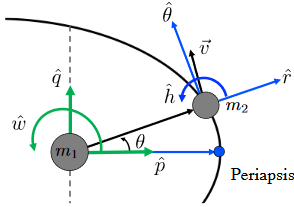
\includegraphics[width=0.5\linewidth]{Figures/perifocal_plane.png}
    
    \textbf{Kepler's Law:} A line joining a planet and the Sun sweep out equal areas during equal intervals of time.\par 
    \textbf{Elliptical Orbits:} $\mathbb{P}=2\pi\sqrt{\frac{a^3}{\mu}}$, $\varepsilon<0$\par
    \textbf{Mean Motion:} $n=\sqrt{\frac{\mu}{a^3}}$ - mean angular rate of motion\par 
    \textbf{Circular Orbits:}
    \begin{itemize}
        \itemsep0em
        \item $r = a$, $\vec{v} \perp \vec{r}$, and $\gamma = 0$ everywhere
        \item $v_c=\sqrt{\frac{\mu}{r}}$
    \end{itemize}
    \textbf{Parabolic Orbits:}
    \begin{itemize}
        \itemsep0em
        \item $e=1$, $a=\inf$, $r_a=$ undefined
        \item Conic equation applies still
        \item $p = \frac{h^2}{\mu}$
        \item $\varepsilon=0$ everywhere
        \item $v = \sqrt{\frac{2\mu}{r}}=v_{esc}$
    \end{itemize}
    \textbf{Hyperbolic Orbits:}
    \begin{itemize}
        \itemsep0em
        \item $v>v_{esc}$, $e>1$, $\varepsilon>0$, $a<0$
        \item $r_p=|a|(e-1)$
        \item $p=|a|(e^2-1)=a(1-e^2)$
        \item $r=\frac{a(1-e^2)}{1+e\cos{\theta}}=\frac{|a|(e^2-1)}{1+e\cos{\theta}}$
        \item at $r = \infty$, $\varepsilon = \frac{-\mu}{2a}=\frac{v^2_{\infty}}{2}\rightarrow v_{\infty}=\sqrt{\frac{\mu}{|a|}}$
        \item $\theta_{\infty} = \pm\cos^{-1}\left({\frac{-1}{e}}\right)$
        \item $v^2=v^2_{esc}+v^2_{\infty}$
        \item turning angle: $\frac{\delta}{2}+90^\circ=\theta_\infty$, $\delta = 2\sin^{-1}({\frac{1}{e}})$
    \end{itemize}
    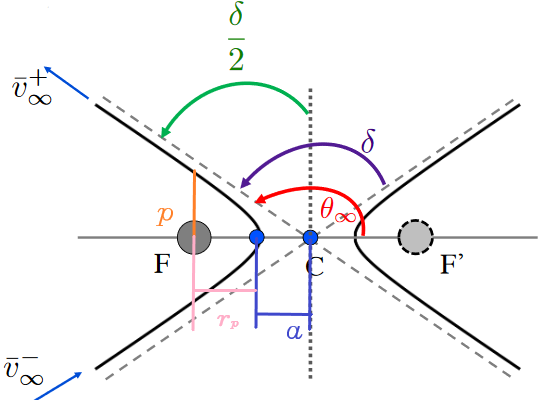
\includegraphics[width=0.5\linewidth]{Figures/hyperbolic_orbit.png}
    \subsection*{The Anomalies}
<<<<<<< HEAD


\end{multicols*}  
=======
    Vis-Viva Equation: $v=\sqrt{\frac{2\mu}{r}-\frac{\mu}{a}}$\par 
    True Anomaly:
\end{multicols*}  



>>>>>>> eefe2b0 (Begins Orbital Exam 1 crib sheet.)
=======


\end{multicols*}  
>>>>>>> c99cbd9 (Finishes the different types of orbits and their properties.)
\end{document}